\documentclass[10pt]{beamer}

%packages
\usepackage{babel}
\usepackage[utf8]{inputenc}
\usepackage{amsmath,tabu}
\usepackage{color}
\usepackage{tikz}
\usetikzlibrary{matrix,chains,positioning,decorations.pathreplacing,arrows}
\usetikzlibrary{calc,shadings}
\usepackage{pgfplots}
\usepackage{colortbl}
\usepackage{eurosym}
\usepackage{mathtools}
\usepackage{listings}

%definitions
\usepackage{algorithm,algorithmic}

%theme
\usetheme{Dresden}
\usecolortheme{rose}
\useoutertheme{tree}

%environments
\newenvironment{ExampleGer}{\begin{exampleblock}{Beispiel}}{\end{exampleblock}}

\newenvironment{customlegend}[1][]{%
	\begingroup
	% inits/clears the lists (which might be populated from previous
	% axes):
	\csname pgfplots@init@cleared@structures\endcsname
	\pgfplotsset{#1}%
}{%
	% draws the legend:
	\csname pgfplots@createlegend\endcsname
	\endgroup
}%

%definitions
\def\addlegendimage{\csname pgfplots@addlegendimage\endcsname}
% definition to insert numbers
\pgfkeys{/pgfplots/number in legend/.style={%
		/pgfplots/legend image code/.code={%
			\node at (0.295,-0.0225){#1};
		},%
	},
}

%general
\title{A Deep Neural Network Approach to Splice Site Prediction}
\author{Tilman Hinnerichs}
\institute{Knowledge Mining Lab -- KAUST}
\date{October 3, 2019}

%presentation
\expandafter\def\expandafter\insertshorttitle\expandafter{%
	\insertshorttitle\hspace{7cm}%
	\insertframenumber\,/\,\inserttotalframenumber
}
\begin{document}
	
\begin{frame}
	\titlepage
\end{frame}

\begin{frame}{Outline}
	\setbeamertemplate{section in toc}[sections numbered]
	\tableofcontents
\end{frame}

\section{Problem Description}
\begin{frame}{Problem Description}
	\begin{figure}[ht]
		\centering
		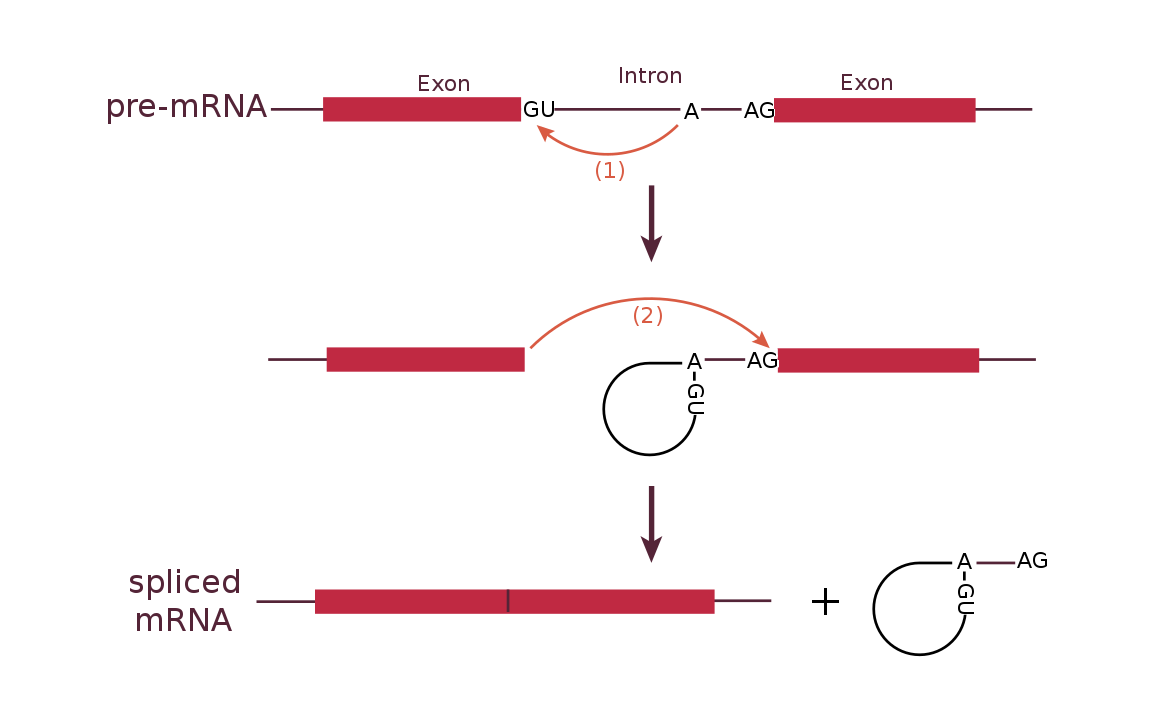
\includegraphics[width = 0.85\textwidth]{RNA_splicing_reaction.png}
		\caption{RNA splicing reaction (en.wikipedia.org)}
	\end{figure}
\end{frame}

\begin{frame}{Problem Description}
	
	\large Splice site prediction on Arabidopsis thaliana genome
	\vspace{0.5cm}
	\pause
	\begin{exampleblock}{}
		\begin{itemize}
			\item Acceptor site:\\
			\dots CGTATCT\only{\colorbox{green}}<3->{AG}ATG\only{\colorbox{red}}<4->{AG}CA\dots
			\item Donor site:\\
			\dots ATGATTT\only{\colorbox{green}}<3->{GT}GCA\only{\colorbox{red}}<4->{GT}CA\dots
			
		\end{itemize}
	\end{exampleblock}
	
\end{frame}

\section{Dataset description}
\begin{frame}{Dataset description}
	
	\large Example file, e.g., acceptor site
	\begin{align*}
	\begin{bmatrix}
	CT \dots \rotatebox{0}{\footnotesize $ 300 $ nt} \dots AG \dots \rotatebox{0}{\footnotesize $ 300 $ nt} \dots GC\\
	AG \dots \rotatebox{0}{\footnotesize $ 300 $ nt} \dots AG \dots \rotatebox{0}{\footnotesize $ 300 $ nt} \dots TT \\
	GA \dots \rotatebox{0}{\footnotesize $ 300 $ nt} \dots AG \dots \rotatebox{0}{\footnotesize $ 300 $ nt} \dots AA \\[0.2ex]
	\vdots\\
	\rotatebox{90}{\footnotesize$ ~100,000 $ records} \\[-1.3ex]
	\vdots \\[1.4ex]
	TT \dots \rotatebox{0}{\footnotesize $ 300 $ nt} \dots AG \dots \rotatebox{0}{\footnotesize $ 300 $ nt} \dots CC
	\end{bmatrix}
	\end{align*}
\end{frame}

\section{DiProDB database}
\subsection{Application of NN}
\begin{frame}{Next Steps from two weeks ago}
	\begin{itemize}
		\item Adapt convolution techniques from other papers with same goal
		\item Vary pre and post marker nt sequence length
		\item Use DiProDB[Friedel et al., NAR, 2009] for input
		\item Utilize electron io interaction potential (EIIP) for prediction
	\end{itemize}
\end{frame}

\begin{frame}{Application of NN to the DiProDB data}
	\begin{itemize}
		\item DiProDB is database for the physicochemical properties of dinucleotides (127 entries)
		\item Applied PCA yielding 15 dimensions
	\end{itemize}
	\pause
		\begin{figure}
		\small
		\centering
		\begingroup
		\def\arraystretch{1.2}
		\begin{tabular}{|l|r|r|r|r|r|r|r|r|}
			\hline
			Approach & Samples & Depth & \multicolumn{3}{|c|}{Acceptor} & \multicolumn{3}{c|}{Donor} \\
			\cline{4-9}
			&&& Acc. & Prec. & Rec. & Acc. & Prec. & Rec. \\
			\hline
			DiProDB & 40,000 & 7 & 92.38 & 92.1 & 93.5 & 93.6 & 92.9 & 93.6 \\
			DiProDB & 40,000 & 9 & 92.28 & 90.4 & 94.2 & 93.4 & 92.0 & 93.9 \\
			
			\hline  
		\end{tabular}
		\endgroup
	\end{figure}
\end{frame}

\begin{frame}[fragile]
	\tiny
	\begin{lstlisting}[frame=none]
		DiProDB BINARY CLASSIFICATION APPROACH
		Data shape: (40000, 601, 15)
		_________________________________________________________________
		Layer (type)                 Output Shape              Param #   
		=================================================================
		input_10 (InputLayer)        (None, 601, 15)           0         
		_________________________________________________________________
		flatten_10 (Flatten)         (None, 9015)              0         
		_________________________________________________________________
		dense_46 (Dense)             (None, 150)               1352400   
		_________________________________________________________________
		dropout_37 (Dropout)         (None, 150)               0         
		_________________________________________________________________
		dense_47 (Dense)             (None, 80)                12080     
		_________________________________________________________________
		dropout_38 (Dropout)         (None, 80)                0         
		_________________________________________________________________
		dense_48 (Dense)             (None, 30)                2430      
		_________________________________________________________________
		dropout_39 (Dropout)         (None, 30)                0         
		_________________________________________________________________
		dense_49 (Dense)             (None, 10)                310       
		_________________________________________________________________
		dropout_40 (Dropout)         (None, 10)                0         
		_________________________________________________________________
		dense_50 (Dense)             (None, 1)                 11        
		=================================================================
		
	
	\end{lstlisting}
\end{frame}

\subsection{Application of CNN}
\begin{frame}{Application of CNN to the DiProDB data}
	\begin{itemize}
		\item Convolutional NN to adapt ideas from other papers
	\end{itemize}
	\pause
	\begin{figure}
		\small
		\centering
		\begingroup
		\def\arraystretch{1.2}
		\begin{tabular}{|l|r|r|r|r|r|r|r|r|}
			\hline
			Approach  & \multicolumn{2}{c}{Layers} & \multicolumn{3}{|c|}{Acceptor} & \multicolumn{3}{c|}{Donor} \\
			\cline{2-9}
			&Conv. & Others & Acc. & Prec. & Rec. & Acc. & Prec. & Rec. \\
			\hline
			CNN DPDB & 4 & 5 & 94.4 & 95.4 & 94.6 & 94.9 & 94.4 & 94.7 \\
			CNN DPDB & 4 & 7 & 93.5 & 93.3 & 94.5 & 94.0 & 94.0 & 93.3 \\
			CNN DPDB & 6 & 5 & 94.0 & 93.9 & 94.9 & 94.2 & 95.4 & 91.6 \\
			CNN DPDB & 6 & 5 & 94.4 & 97.0 & 93.8 & 95.2 & 96.5 & 93.7 \\
			SpliceRover & 4 & 2 & 96.1 & 93.9 & 97.4 & 95.4 & 95.6 & 96.7 \\
			CNN DPDB(*) & 2 & 4 & 94.3 & 95.6 & 94.3 & 95.3 & 96.9 & 94.4 \\
			
			\hline  
		\end{tabular}
		\endgroup
	\end{figure}
	SpliceRover[Zuallaert et al., 2018]

\end{frame}

\begin{frame}[fragile]
	\tiny
	\begin{lstlisting}
		DiProDB: BINARY CLASSIFICATION APPROACH
		Data shape: (40000, 601, 15, 1)
		Epochs: 5, Batch size: 500
		Model: "model_10"
		_________________________________________________________________
		Layer (type)                 Output Shape              Param #   
		=================================================================
		input_10 (InputLayer)        (None, 601, 15, 1)        0         
		_________________________________________________________________
		conv2d_28 (Conv2D)           (None, 599, 1, 32)        1472      
		_________________________________________________________________
		max_pooling2d_28 (MaxPooling (None, 299, 1, 32)        0         
		_________________________________________________________________
		conv2d_29 (Conv2D)           (None, 297, 1, 64)        6208      
		_________________________________________________________________
		max_pooling2d_29 (MaxPooling (None, 148, 1, 64)        0         
		_________________________________________________________________
		conv2d_30 (Conv2D)           (None, 146, 1, 128)       24704     
		_________________________________________________________________
		max_pooling2d_30 (MaxPooling (None, 48, 1, 128)        0         
		_________________________________________________________________
		flatten_10 (Flatten)         (None, 6144)              0         
		_________________________________________________________________
		dense_28 (Dense)             (None, 64)                393280    
		_________________________________________________________________
		dropout_19 (Dropout)         (None, 64)                0         
		_________________________________________________________________
		dense_29 (Dense)             (None, 64)                4160      
		_________________________________________________________________
		dropout_20 (Dropout)         (None, 64)                0         
		_________________________________________________________________
		dense_30 (Dense)             (None, 1)                 65        
		=================================================================
		
	\end{lstlisting}
\end{frame}

\begin{frame}
	\begin{figure}[ht]
		\centering
		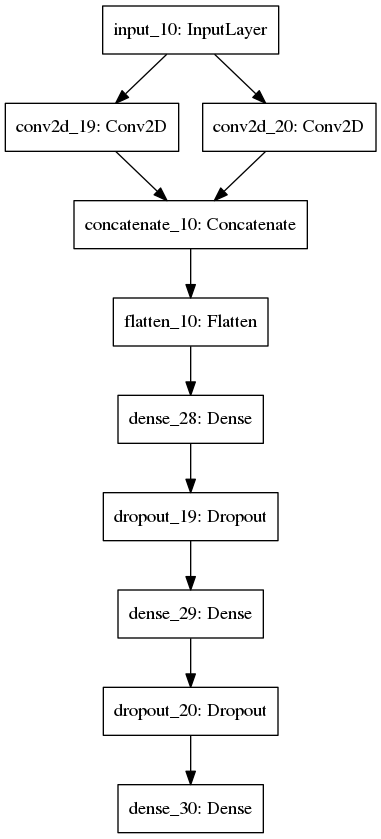
\includegraphics[width = 0.65\textwidth]{../../models/plotted_models/DiProDB_model.png}
	\end{figure}
\end{frame}

\section{Improvements on simple approach}
\begin{frame}{Improvements on simple approach}
	Applying convolutional models to one hot encoding of
	\begin{itemize}
		\item single nucleotides
		\begin{figure}
			\small
			\centering
			\begingroup
			\def\arraystretch{1.2}
			\begin{tabular}{|l|r|r|r|r|r|r|r|}
				\hline
				Approach  & Samples & \multicolumn{3}{c|}{Acceptor} & \multicolumn{3}{c|}{Donor} \\
				\cline{3-8}
				& & Acc. & Prec. & Rec. & Acc. & Prec. & Rec. \\
				\hline
				Simple & 200000 & 94.5 & 95.6 & 93.3 & 95.3 & 96.7 & 94.5 \\
				
				\hline  
			\end{tabular}
			\endgroup
		\end{figure}
		\item trinucleotides
		\begin{figure}
			\small
			\centering
			\begingroup
			\def\arraystretch{1.2}
			\begin{tabular}{|l|r|r|r|r|r|r|r|}
				\hline
				Approach  & Samples & \multicolumn{3}{c|}{Acceptor} & \multicolumn{3}{c|}{Donor} \\
				\cline{3-8}
				& & Acc. & Prec. & Rec. & Acc. & Prec. & Rec. \\
				\hline
				Simple & 200000 & 94.6 & 93.3 & 96.7 & 95.0 & 92.5 & 96.3 \\
				
				\hline  
			\end{tabular}
			\endgroup
		\end{figure}
	\end{itemize}
\end{frame}

\begin{frame}{Single nucleotides model}
	\begin{figure}[ht]
		\centering
		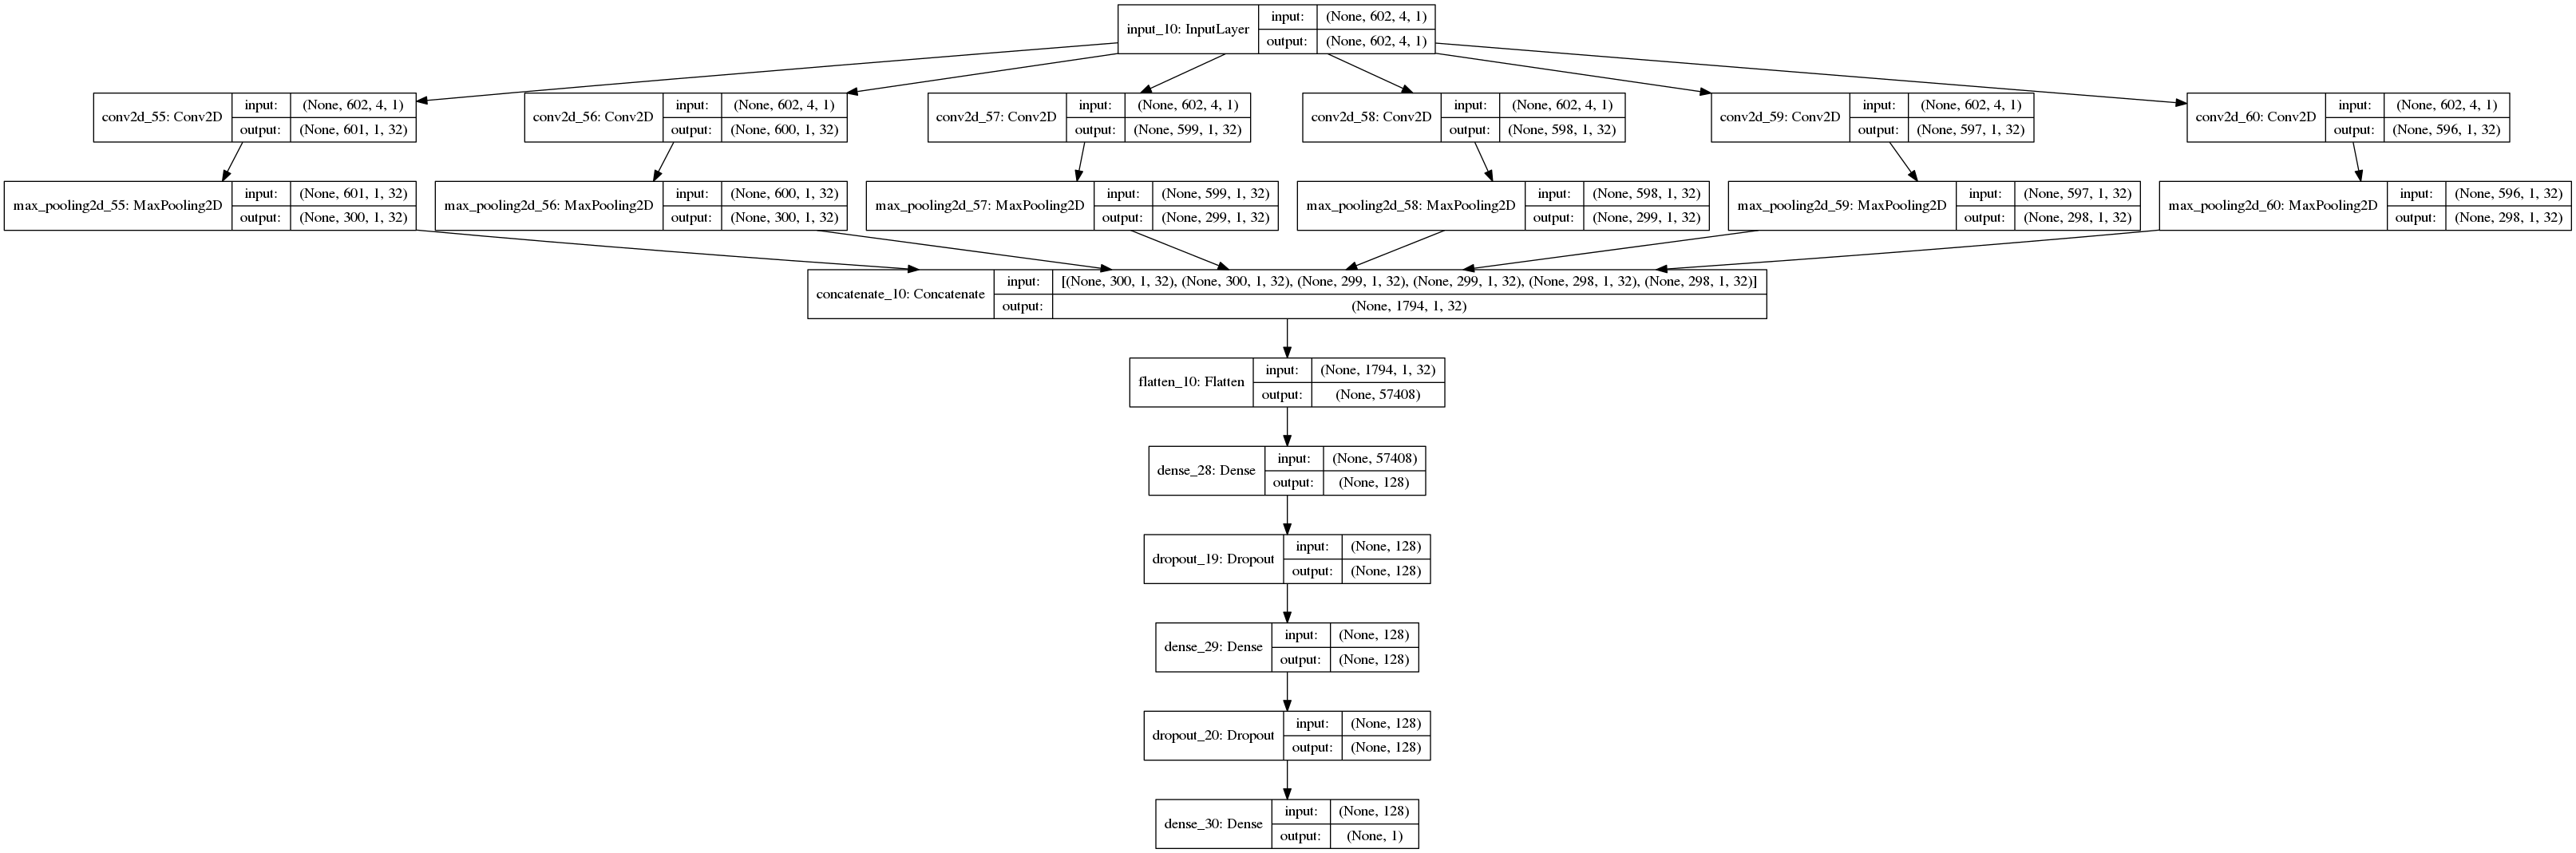
\includegraphics[width = 1.05\textwidth]{../../models/plotted_models/simple_model.png}
		\caption{Convolutional model with filter sizes (2x4), \dots, (7x4)}
	\end{figure}
\end{frame}

\begin{frame}{Trinucleotides model}
	\begin{figure}[ht]
		\centering
		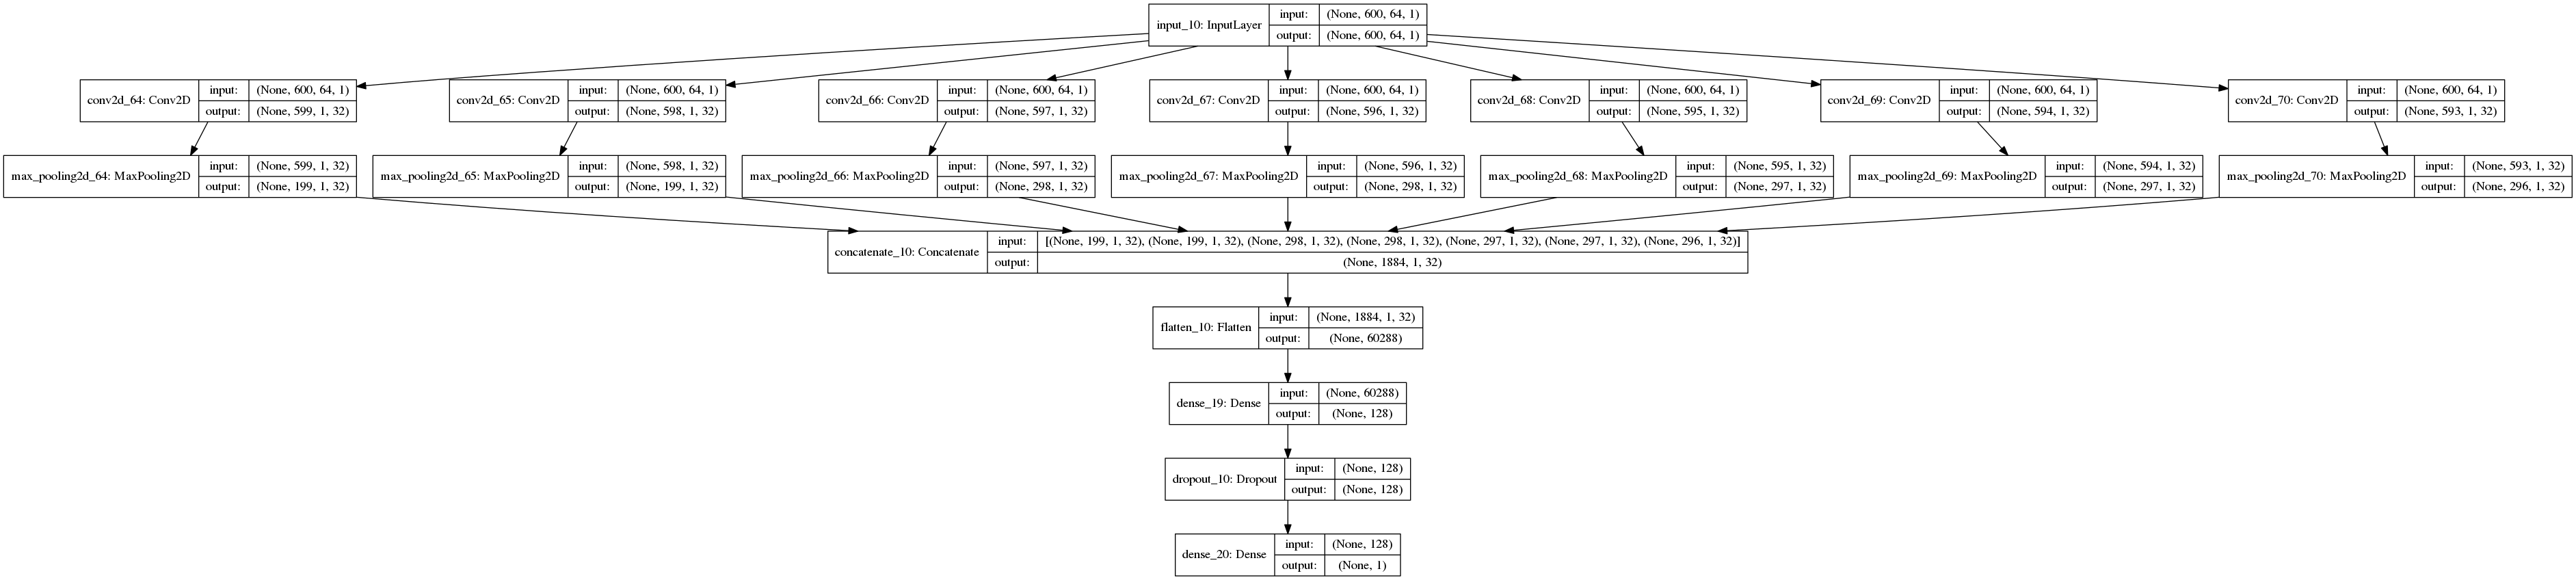
\includegraphics[width = 1.05\textwidth]{../../models/plotted_models/trint_model_2019-10-02_14-53-06.png}
		\caption{Convolutional model with filter sizes (2 x 64), \dots, (8x64)}
	\end{figure}
\end{frame}

\section{repDNA}
\begin{frame}{repDNA (Liu, 2014)}
	A \glqq Python package to generate various modes of feature vectors for DNA sequences\grqq:
	\begin{block}{repDNA content}
		\begin{itemize}
			\item Nucleic acid composition
			\begin{itemize}
				\item kmer
				\item Increment of diversity (ID)
			\end{itemize}
			\item Autocorrelation
			\begin{itemize}
				\item Dinucleotide-based auto covariance (DAC)
				\item Dinucleotide-based cross covariance (DCC)
				\item Dinucleotide-based auto-cross covariance (DACC)
				\item Trinucleotide-based auto covariance (TAC)
				\item Trinucleotide-based cross covariance (TCC)
				\item Trinucleotide-based auto-cross covariance (TACC)
			\end{itemize}
		\end{itemize}
	\end{block}
\end{frame}

\begin{frame}{repDNA (Liu, 2014)}
	\begin{block}{repDNA content}
		\begin{itemize}
			\item Pseudo nucleotide composition
			\begin{itemize}
				\item Pseudo dinucleotide composition (PseDNC)
				\item Pseudo k-tupler nucleotide composition (PseKNC)
				\item Parallel correlation pseudo dinucleotide composition (PC-PseDNC)
				\item Parallel correlation pseudo trinucleotide composition (PC-PseTNC)
				\item Series correlation pseudo dinucleotide composition (SC-PseDNC)
				\item Series correlation pseudo trinucleotide composition (SC-PseTNC)
			\end{itemize}
		\end{itemize}
	\end{block}
	\pause
	\begin{itemize}
		\item Build model for each encoding and reuse filters for overall model
	\end{itemize}
\end{frame}

\begin{frame}{Classifier model on repDNA features: Results}
	\begin{figure}
		\small
		\centering
		\begingroup
		\def\arraystretch{1.2}
		\begin{tabular}{|l|r|r|r|r|r|r|r|}
			\hline
			Approach  & Samples & \multicolumn{3}{c|}{Acceptor} & \multicolumn{3}{c|}{Donor} \\
			\cline{3-8}
			& & Acc. & Prec. & Rec. & Acc. & Prec. & Rec. \\
			\hline
			IDkmer & 40000 & 75.4 & 71.4 & 78.5 & 73.2 & 69.6 & 76.5 \\
			DAC & 40000 & 74.1 & 74.2 & 74.3 & 72.9 & 72.2 & 73.2 \\
			DCC & 40000 & 75.1 & 80.0 & 77.7 & 74.5 & 75.2 & 80.0 \\
			PC-PseDNC & 40000 & 78.0 & 76.5 & 80.1 & 76.4 & 75.1 & 77.9 \\
			PC-PseTNC & 40000 & 80.5 & 76.1 & 84.2 & 78.8 & 76.9 & 81.6 \\
			SC-PseDNC & 40000 & 79.2 & 74.5 & 82.4 & 77.5 & 77.0 & 78.8 \\
			SC-PseTNC & 40000 & 80.6 & 76.3 & 84.8 & 78.7 & 77.3 & 81.5\\
			
			\hline  
		\end{tabular}
		\endgroup
	\end{figure}
\end{frame}

\begin{frame}{Classifier model on repDNA features: IDkmer}
	\begin{figure}[ht]
		\centering
		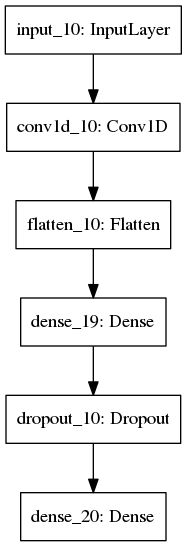
\includegraphics[width = 0.35\textwidth]{../../models/plotted_models/IDkmer_model.png}
	\end{figure}
\end{frame}

\begin{frame}{Classifier model on repDNA features: DAC/DCC}
	\begin{figure}[ht]
		\centering
		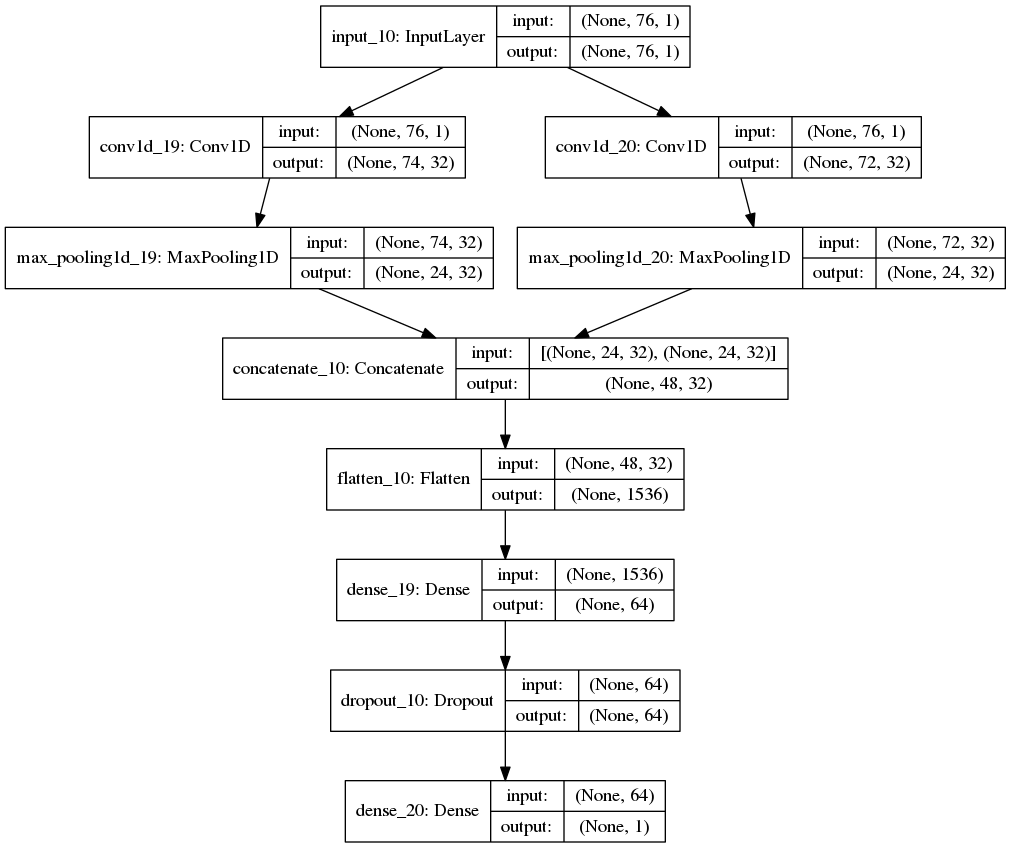
\includegraphics[width = 0.75\textwidth]{../../models/plotted_models/dac_model.png}
	\end{figure}
\end{frame}

\begin{frame}{Classifier model on repDNA features: PseNAC}
	\begin{figure}[ht]
		\centering
		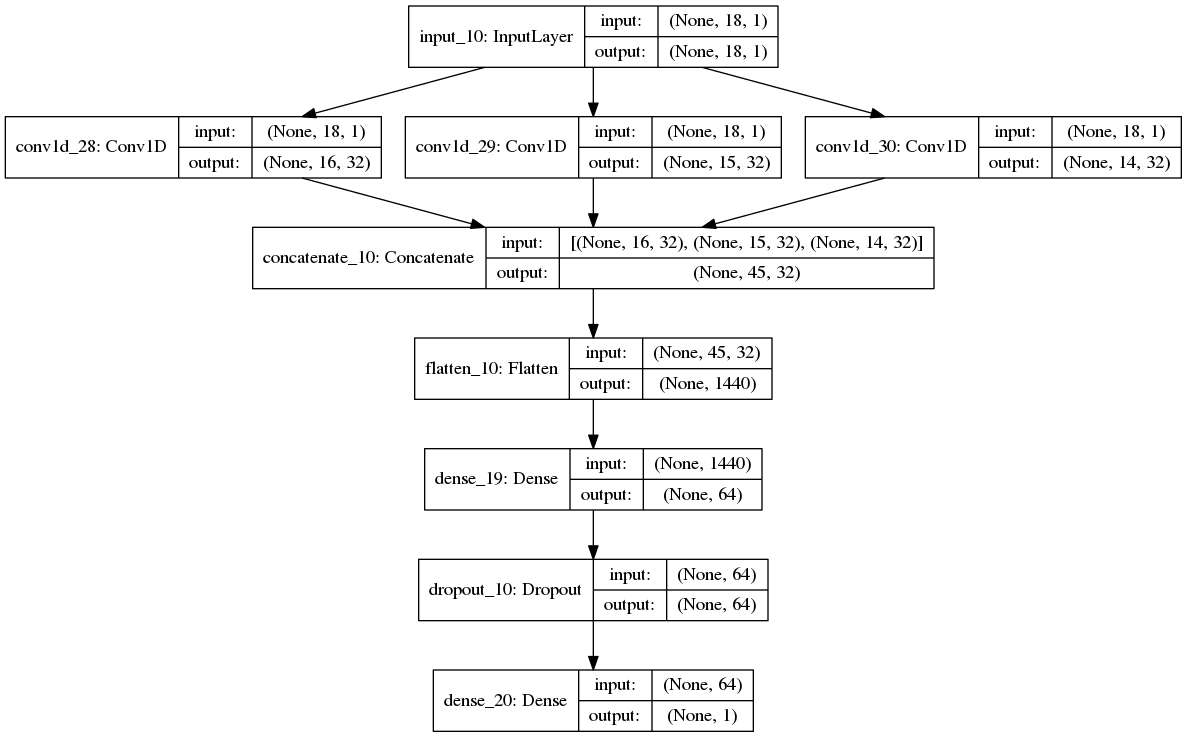
\includegraphics[width = 0.95\textwidth]{../../models/plotted_models/PC_PseDNC_model.png}
	\end{figure}
\end{frame}

\subsection{Funnel}
\begin{frame}{Funneling method: Model}
	\begin{figure}[ht]
		\centering
		\tikzset{%
			every neuron/.style={
				circle,
				draw,
				minimum size=0.5cm
			},
			neuron missing/.style={
				draw=none, 
				scale=4,
				text height=0.333cm,
				execute at begin node=\color{black}$\vdots$
			},
		}
		
		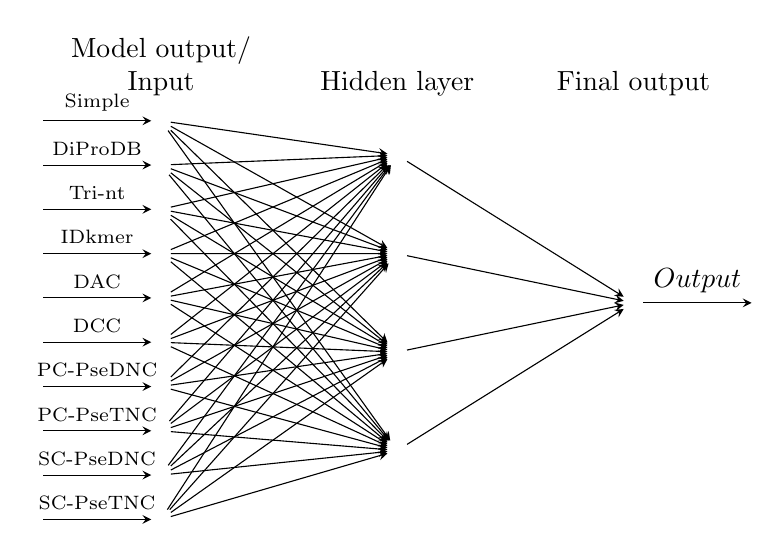
\begin{tikzpicture}[x=1.5cm, y=1.25cm, >=stealth]
		
		\foreach \m/\l [count=\y] in {1,2,3,4,5,6,7,8,9,10}
		\node [every neuron/.try, neuron \m/.try] (input-\m) at (0,2.3-0.45*\y) {};
		
		\foreach \m [count=\y] in {1,2,3,4}
		\node [every neuron/.try, neuron \m/.try ] (hidden-\m) at (2,2.5-\y) {};
		
		\foreach \m [count=\y] in {1}
		\node [every neuron/.try, neuron \m/.try ] (output-\m) at (4,0) {};
		
		%\foreach \l [count=\i] in {1, 2,3,4,5,6,7,8,9,10}
		%\draw [<-] (input-\i) -- ++(-1,0)
		%node [above, midway] {$I_{\l}$};
		
		\draw [<-] (input-1) -- ++(-1,0)
		node [above, midway] {\scriptsize Simple};
		\draw [<-] (input-2) -- ++(-1,0)
		node [above, midway] {\scriptsize DiProDB};
		\draw [<-] (input-3) -- ++(-1,0)
		node [above, midway] {\scriptsize Tri-nt};
		\draw [<-] (input-4) -- ++(-1,0)
		node [above, midway] {\scriptsize IDkmer};
		\draw [<-] (input-5) -- ++(-1,0)
		node [above, midway] {\scriptsize DAC};
		\draw [<-] (input-6) -- ++(-1,0)
		node [above, midway] {\scriptsize DCC};
		\draw [<-] (input-7) -- ++(-1,0)
		node [above, midway] {\scriptsize PC-PseDNC};
		\draw [<-] (input-8) -- ++(-1,0)
		node [above, midway] {\scriptsize PC-PseTNC};
		\draw [<-] (input-9) -- ++(-1,0)
		node [above, midway] {\scriptsize SC-PseDNC};
		\draw [<-] (input-10) -- ++(-1,0)
		node [above, midway] {\scriptsize SC-PseTNC};
		
		\foreach \l [count=\i] in {1}
		\draw [->] (output-\i) -- ++(1,0)
		node [above, midway] {$Output$};
		
		\foreach \i in {1,...,10}
		\foreach \j in {1,...,4}
		\draw [->] (input-\i) -- (hidden-\j);
		
		\foreach \i in {1,...,4}
		\foreach \j in {1,...,1}
		\draw [->] (hidden-\i) -- (output-\j);
		
		%\foreach \l [count=\x from 0] in {Input, Hidden, Ouput}
		\node [align=center, above] at (0*2,2) {Model output/\\Input};
		\node [align=center, above] at (1*2,2) {Hidden layer};
		\node [align=center, above] at (2*2,2) {Final output};

		\end{tikzpicture}
	\end{figure}
\end{frame}

\begin{frame}{Funneling method: Results}
	\begin{figure}
		\footnotesize
		\centering
		\begingroup
		\def\arraystretch{1.2}
		\begin{tabular}{|r|r|r|r|r|r|r|r|r|r|r|}
			\hline
			 S&D & IK & Pse & D & \multicolumn{3}{c|}{Acceptor} & \multicolumn{3}{c|}{Donor} \\
			\cline{6-11}
			&&&&& Acc. & Prec. & Rec. & Acc. & Prec. & Rec. \\
			\hline
			X & X &&& & 97.7 & 98.1 & 96.7 & --- & --- & --- \\
			\hline
			X & X & X & & & 97.7 & 98.1 & 96.7 & --- & --- & --- \\
			\hline
			X & X & X & X & & 97.6 & 98.2 & 96.2 & --- & --- & --- \\
			\hline
			X & X & X & X & X & 97.5 & 98.2 & 96.5 & 97.4 & 97.3 & 96.3 \\
			\hline
			
			
			
			\hline  
		\end{tabular}
		\endgroup
	\end{figure}
\end{frame}

\section{Next Steps}
\begin{frame}{Next steps}
	\begin{itemize}
		\item Follow improvements of SpliceRover
		\item repDNA (Liu et al., 2015) for different embeddings of the sequences
		\item Train CNN on all embeddings
		\item Freeze convolutional layers and funnel them into DNN
	\end{itemize}
\end{frame}

\begin{frame}{Citations}
	\footnotesize
	\begin{itemize}
		\item Liu B, Liu F, Fang L, Wang X, Chou K-C.repDNA: a Python package to generate various modes of feature vectors for DNA sequences by incorporating user-defined physicochemical properties and sequence-order effects. Bioinformatics 2015;31(8):1307-1309.
		\item Jasper Zuallaert, Fréderic Godin, Mijung Kim, Arne Soete, Yvan Saeys, Wesley De Neve, SpliceRover: interpretable convolutional neural networks for improved splice site prediction, Bioinformatics, Volume 34, Issue 24, 15 December 2018, Pages 4180–4188, https://doi.org/10.1093/bioinformatics/bty497
	\end{itemize}
\end{frame}

\end{document}